\chapter*{Dodatak: Prikaz aktivnosti grupe}
		\addcontentsline{toc}{chapter}{Dodatak: Prikaz aktivnosti grupe}
		
		\section*{Dnevnik sastajanja}
		\begin{packed_enum}
			\item  sastanak
			
			\item[] \begin{packed_item}
				\item Datum: 14.10.2022 
				\item Prisustvovali: Mateja Golec, Luka Nola, Nina Đurić, Lara Đaković, Lucija Domić, Ana Vrabec, Karlo Boroš
				\item Teme sastanka: 
				\begin{packed_item}
					\item  upoznavanje
					\item  dogovor oko korištenih tehnologija
					\item  dogovor načina komunikacije
				\end{packed_item}
			\end{packed_item}
			

			\item  sastanak
			
			\item[] \begin{packed_item}
				\item Datum: 20.10.2022 
				\item Prisustvovali: Mateja Golec, Luka Nola, Nina Đurić, Lara Đaković, Lucija Domić, demonstrator, asistent
				\item Teme sastanka:
				\begin{packed_item}
					\item  sastnak s asistentom i demonstratorom
					\item  dogovor funkcionalnosti i rješavanje osnovnih dilema
					\item  dogovor oko korištenih tehnologija
					\item  analiza zadatka
				\end{packed_item}
			\end{packed_item}
			
			\item  sastanak
			\item[] \begin{packed_item}
				\item Datum:  24.10.2022.
				\item Prisustvovali: Mateja Golec, Luka Nola, Nina Đurić, Lara Đaković, Lucija Domić, Ana Vrabec, Karlo Boroš
				\item Teme sastanka:
				\begin{packed_item}
					\item  dogovor oko pisanja dokumentacije i podjele poslova u početnoj fazi
				\end{packed_item}
			\end{packed_item}
			
			\item  sastanak
			\item[] \begin{packed_item}
				\item Datum:  25.10.2022.
				\item Prisustvovali: Luka Nola, Lara Đaković
				\item Teme sastanka:
				\begin{packed_item}
					\item  izrada ER dijagrama baze podataka
				\end{packed_item}
			\end{packed_item}

			\item  sastanak
			\item[] \begin{packed_item}
				\item Datum: 25.10.2022.
				\item Prisustvovali: Mateja Golec, Luka Nola, Nina Đurić, Lara Đaković, Lucija Domić, Ana Vrabec, Karlo boroš
				\item Teme sastanka:
				\begin{packed_item}
					\item  definiranje obrazaca uporabe
					\item  definiranje funkcionalnih zahtjeva
					\item  raspodjela poslova oko izrade obrazaca uporabe, funkcionalnih zahtjeva i opisa zadatka
				\end{packed_item}
			\end{packed_item}

			\item  sastanak
			\item[] \begin{packed_item}
				\item Datum: 27.10.2022.
				\item Prisustvovali: Mateja Golec, Nina Đurić, Lara Đaković, Luka Nola, asistent
				\item Teme sastanka:
				\begin{packed_item}
					\item  pregled funkcionalnih zahtjeva
					\item  pregled obrazaca uporabe
					\item  pregled opisa
					\item  razješavanje dilema za ER dijagram baze podataka
				\end{packed_item}
			\end{packed_item}

			\item  sastanak
			\item[] \begin{packed_item}
				\item Datum: 31.10.2022.
				\item Prisustvovali: Mateja Golec, Nina Đurić, Lara Đaković, Lucija Domić, Ana Vrabec, Karlo Boroš
				\item Teme sastanka:
				\begin{packed_item}
					\item  pregled obrazaca uporabe
					\item  upoznavanje sa latexom
					\item  dogovor za crtanje dijagrama obrazaca uporabe
				\end{packed_item}
			\end{packed_item}

			\item  sastanak
			\item[] \begin{packed_item}
				\item Datum: 4.11.2022.
				\item Prisustvovali: Mateja Golec, Luka Nola, Nina Đurić, Lara Đaković, Lucija Domić, Ana Vrabec, Karlo Boroš
				\item Teme sastanka:
				\begin{packed_item}
					\item  objašnjavanje radnog okruženja i pokretatanje stranice
					\item  definiranje sekvencijskih dijagrama
					\item  raspodjela poslova oko baze podataka i sekvencijskih dijagrama
				\end{packed_item}
			\end{packed_item}

			\item  sastanak
			\item[] \begin{packed_item}
				\item Datum: 9.11.2022.
				\item Prisustvovali: Mateja Golec, Luka Nola, Nina Đurić, Lara Đaković, Lucija Domić, Ana Vrabec, Karlo Boroš
				\item Teme sastanka:
				\begin{packed_item}
					\item  dogovor oko opisa arhitekture
					\item  raspodjela posla i dogovor oko dijagrama razreda
					\item  raspodjela posla i dogovor za autentikaciju i autorizaciju
				\end{packed_item}
			\end{packed_item}

			\item  sastanak
			\item[] \begin{packed_item}
				\item Datum: 10.11.2022.
				\item Prisustvovali: Mateja Golec, Luka Nola, Nina Đurić, Lucija Domić, Ana Vrabec, asistent
				\item Teme sastanka:
				\begin{packed_item}
					\item  pregled dokumentacije
					\item  razrješavanje pitanja u vezi baze,  autorizacije i klasnih dijagrama
				\end{packed_item}
			\end{packed_item}

			\item  sastanak
			\item[] \begin{packed_item}
				\item Datum: 14.11.2022.
				\item Prisustvovali: Mateja Golec, Luka Nola, Nina Đurić, Lara Đaković, Lucija Domić, Ana Vrabec, Karlo Boroš
				\item Teme sastanka:
				\begin{packed_item}
					\item  pregled rada aplikacije
					\item  dovršavanje klasnih dijagrama
				\end{packed_item}
			\end{packed_item}

			\item  sastanak
			\item[] \begin{packed_item}
				\item Datum: 16.11.2022.
				\item Prisustvovali: Mateja Golec, Luka Nola, Nina Đurić, Lara Đaković, Lucija Domić, Ana Vrabec, Karlo Boroš
				\item Teme sastanka:
				\begin{packed_item}
					\item  pregled rada aplikacije
					\item  pregled dokumentacije
				\end{packed_item}
			\end{packed_item}	
			
			
			\item  sastanak
			\item[] \begin{packed_item}
				\item Datum: 15.12.2022.
				\item Prisustvovali: Mateja Golec, Luka Nola, Nina Đurić, Lara Đaković, Lucija Domić, Ana Vrabec, Karlo Boroš
				\item Teme sastanka:
				\begin{packed_item}
					\item  podjela askova
				\end{packed_item}
			\end{packed_item}

			\item  sastanak
			\item[] \begin{packed_item}
				\item Datum: 4.1.2023.
				\item Prisustvovali: Mateja Golec, Luka Nola, Nina Đurić, Lara Đaković, Lucija Domić, Ana Vrabec, Karlo Boroš
				\item Teme sastanka:
				\begin{packed_item}
					\item  pregled odrađenog posla
					\item  podjela taskova
				\end{packed_item}
			\end{packed_item}

			\item  sastanak
			\item[] \begin{packed_item}
				\item Datum: 9.1.2023.
				\item Prisustvovali: Mateja Golec, Luka Nola, Nina Đurić, Lara Đaković, Lucija Domić, Ana Vrabec, Karlo Boroš
				\item Teme sastanka:
				\begin{packed_item}
					\item  pregled odrađenog posla
					\item  podjela taskova
					\item  dogovor posla za dokumentaciju
				\end{packed_item}
			\end{packed_item}
		\end{packed_enum}
		
		\eject
		\section*{Tablica aktivnosti}
		

			\begin{longtblr}[
					label=none,
				]{
					vlines,hlines,
					width = \textwidth,
					colspec={X[7, l]X[1, c]X[1, c]X[1, c]X[1, c]X[1, c]X[1, c]X[1, c]}, 
					vline{1} = {1}{text=\clap{}},
					hline{1} = {1}{text=\clap{}},
					rowhead = 1,
				} 
				\multicolumn{1}{c|}{} & \multicolumn{1}{c|}{\rotatebox{90}{\textbf{Mateja Golec}}} & \multicolumn{1}{c|}{\rotatebox{90}{\textbf{Karlo Boroš }}} & \multicolumn{1}{c|}{\rotatebox{90}{\textbf{Lucija Domić}}} & \multicolumn{1}{c|}{\rotatebox{90}{\textbf{Lara Đaković}}} & \multicolumn{1}{c|}{\rotatebox{90}{\textbf{Nina Đurić}}} & \multicolumn{1}{c|}{\rotatebox{90}{\textbf{Luka Nola}}} & \multicolumn{1}{c|}{\rotatebox{90}{\textbf{Ana Vrabec}}}  \\
				Upravljanje projektom 		& 20h & 13h & 13h & 14h & 13h & 40h & 16h \\ 
				Opis projektnog zadatka 	&  &  &  &  & 6h &  & \\ 
				
				Funkcionalni zahtjevi       &3h  &  &  &  &  &  &  \\ 
				Opis pojedinih obrazaca 	&  & 5h & 6h & 7h &  &  & 7h \\ 
				Dijagram obrazaca 			&  & 3h & 4h & 4h &  &  & 4h \\ 
				Sekvencijski dijagrami 		&4h  &  &  &  & 2h &  &  \\  
				Opis ostalih zahtjeva 		&  &  &  &  &  &  &  2h \\ 

				Arhitektura i dizajn sustava	 &3h  &  &  &  &  & 2h &  \\ 
				Baza podataka				& 1h & 5h &  & 5h &  & 2h & 5h\\ 
				Dijagram razreda 			&  &  & 3h & 11h & 2h & 2h &  5h \\  
				Dijagram stanja				& 2h &  &  &  &  &  &  \\ 
				Dijagram aktivnosti 		&  & 3h &  &  &  &  &  \\ 
				Dijagram komponenti			&  &  & 5h &  &  &  &  \\ 
				Korištene tehnologije i alati 		& 2h &  &  &  &  &  &  \\ 
				Ispitivanje programskog rješenja 	&  &  &  &  &  &  &  \\ 
				Dijagram razmještaja			&  &  &  &  & 1.5h &  &  \\ 
				Upute za puštanje u pogon 		& 5h &  &  &  &  &  &  \\  
				Dnevnik sastajanja 			&  &  &  & 2h &  &  &3h  \\ 
				Zaključak i budući rad 		&  &  &  & 1.5h &  &  &  \\  
				Popis literature 			&  &  &  &  &  &  &  \\  
				&  &  &  &  &  &  &  \\ \hline 
				\textit{Postavljanje klijentske strane aplikacije} 				&7h  & 9h & 20h &  & 5h & 20h & 20h \\  
				\textit{Postavljanje serverske strane aplikacije} 				&10h  & 3h &  20h &  & 4h & 20h &20h  \\  
				\textit{Konfiguracija infrastrukutre} 				&  &  &  &  &  & 1h &  \\  
				\textit{Izrada modela baze podataka} 		 			&  &  & 10h & 4h &  & 3h & 4h\\  
				\textit{Autorizacija i autentikacija - backend}	&  & 5h & &  &  & 5h &  \\
				\textit{Kreacija modela, migracija i punjenje baze} 							&  &  & 3h &  &  & 2h &  \\ 
				\textit{Kreacija kluba} 							&  &  &  &  &  & 2h &  \\ 
				\textit{Kreacija, uredivanje i pregled korisnika} 							&  &  &  &  &  & 5h &  \\ 
				\textit{Pustanje u pogon (deployment)} 							&  &  &  &  &  & 8h  &  \\
				\textit{Kreacija modela Course i Lesson, migracija, punjenje baze} 							&  &  &  & 10h &  & &  \\
				\textit{Inicijalizacija mape} 							&  &  &  & 13h &  & &  \\
				\textit{Prikaz courseva na karti} 							&  &  &  &17h  &  & &  \\
				\textit{Prikaz Lessona na kalendaru} 							&  &  &  & 10h &  & &  \\
				\textit{Seed adekvatnih podataka u bazu} 							&  &  &  &3h  &  & &  
				\textit{Review} 							&  &  &  &  & 20h & 4h&  \\
				\textit{Kreacija preostalih controllera i rad na projektu}				&15h  & 15h & 15h & 15h & 30h & 30h&  \\
			\end{longtblr}
					
					
		\eject
		\section*{Dijagrami pregleda promjena}
		
		% \textbf{\textit{dio 2. revizije}}\\
		
		% \textit{Prenijeti dijagram pregleda promjena nad datotekama projekta. Potrebno je na kraju projekta generirane grafove s gitlaba prenijeti u ovo poglavlje dokumentacije. Dijagrami za vlastiti projekt se mogu preuzeti s gitlab.com stranice, u izborniku Repository, pritiskom na stavku Contributors.}
		\begin{figure}[H]
			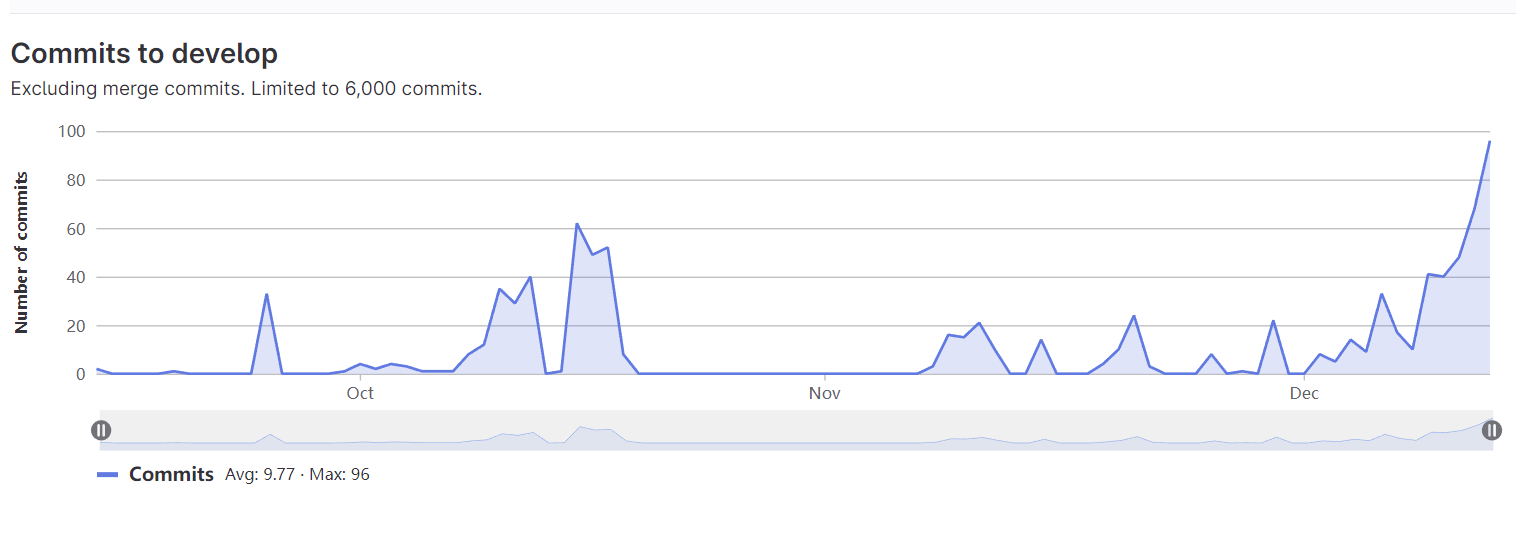
\includegraphics[scale=0.6]{slike/git1.png} %veličina slike u odnosu na originalnu datoteku i pozicija slike
			\centering
			\caption{Aktivnost develop grane 1}
			\label{fig:aktivnost1}
		\end{figure}
		\begin{figure}[H]
			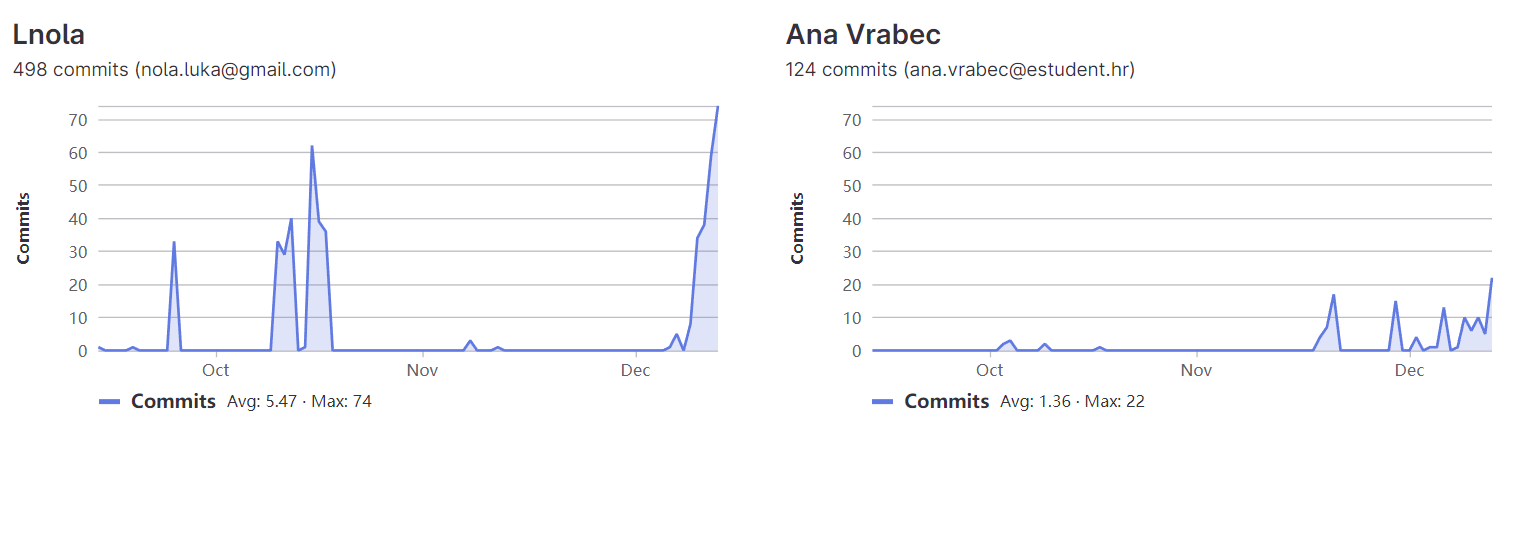
\includegraphics[scale=0.6]{slike/git2.png} %veličina slike u odnosu na originalnu datoteku i pozicija slike
			\centering
			\caption{Aktivnost develop grane 2}
			\label{fig:aktivnost2}
		\end{figure}
		\begin{figure}[H]
			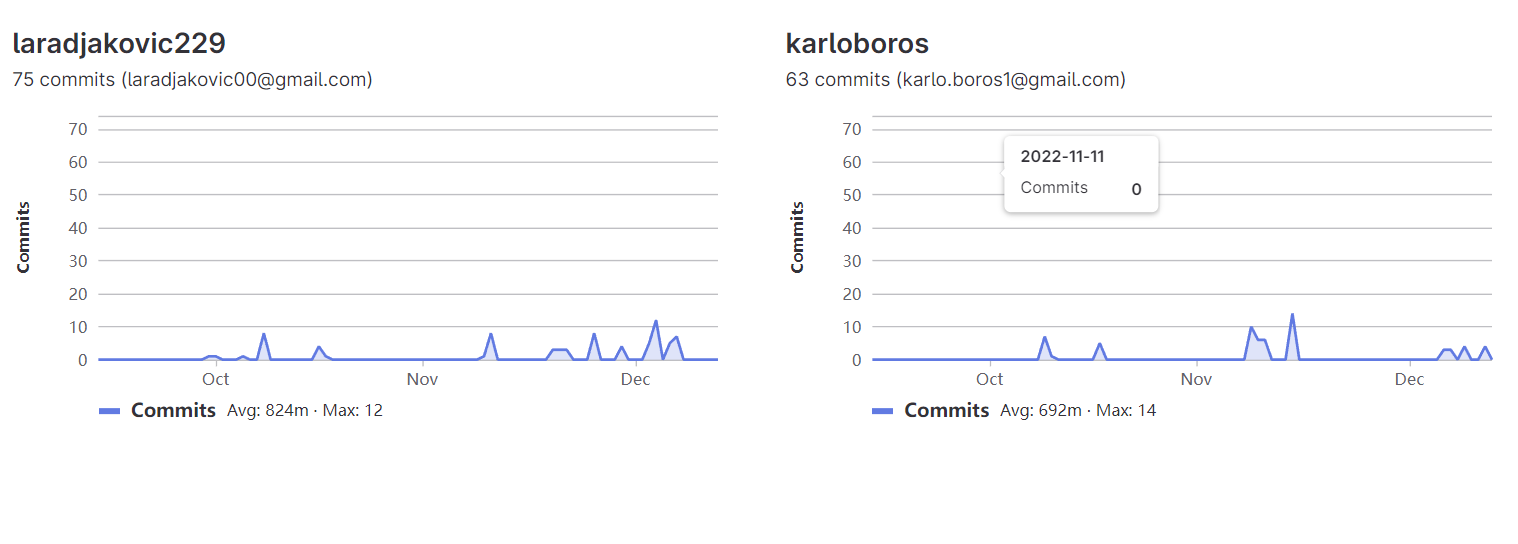
\includegraphics[scale=0.6]{slike/git3.png} %veličina slike u odnosu na originalnu datoteku i pozicija slike
			\centering
			\caption{Aktivnost develop grane 3}
			\label{fig:aktivnost3}
		\end{figure}
		\begin{figure}[H]
			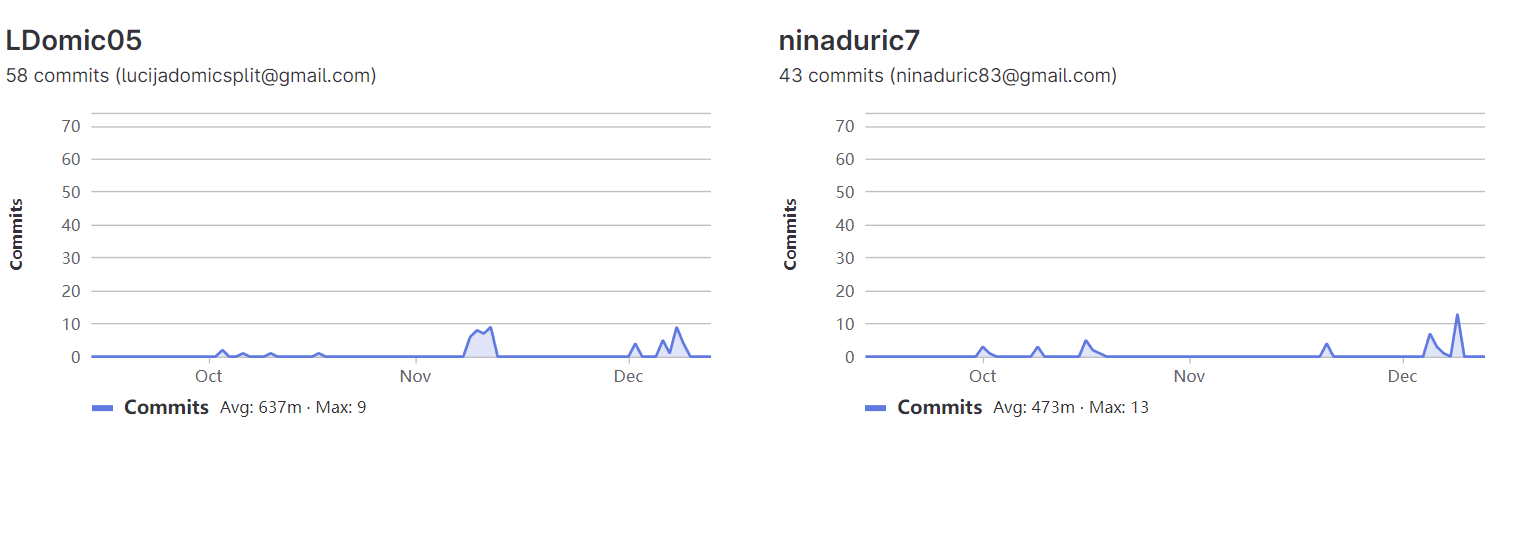
\includegraphics[scale=0.6]{slike/git4.png} %veličina slike u odnosu na originalnu datoteku i pozicija slike
			\centering
			\caption{Aktivnost develop grane 4}
			\label{fig:aktivnost4}
		\end{figure}
		\begin{figure}[H]
			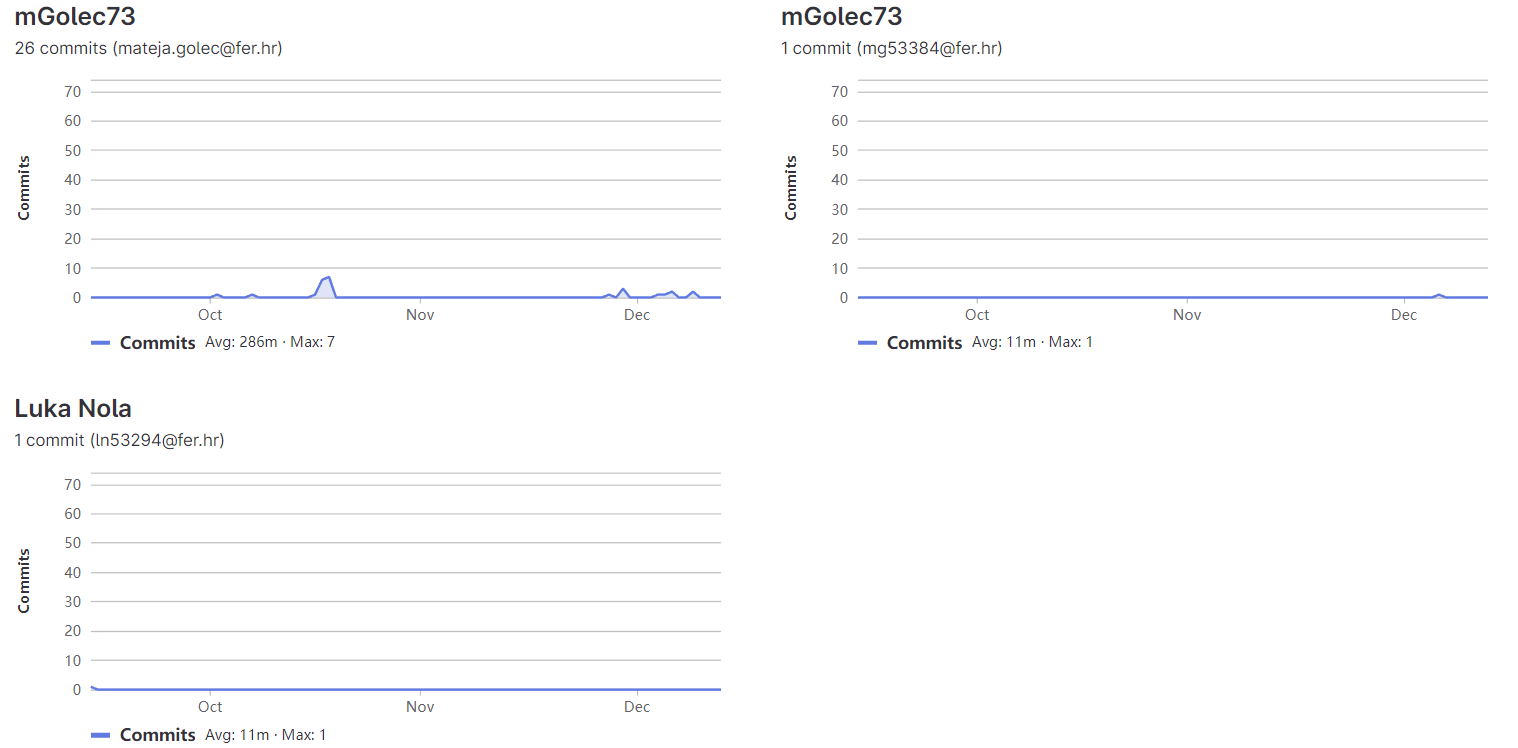
\includegraphics[scale=0.6]{slike/git5.png} %veličina slike u odnosu na originalnu datoteku i pozicija slike
			\centering
			\caption{Aktivnostde develop grane 5}
			\label{fig:aktivnost5}
		\end{figure}
		\begin{figure}[H]
			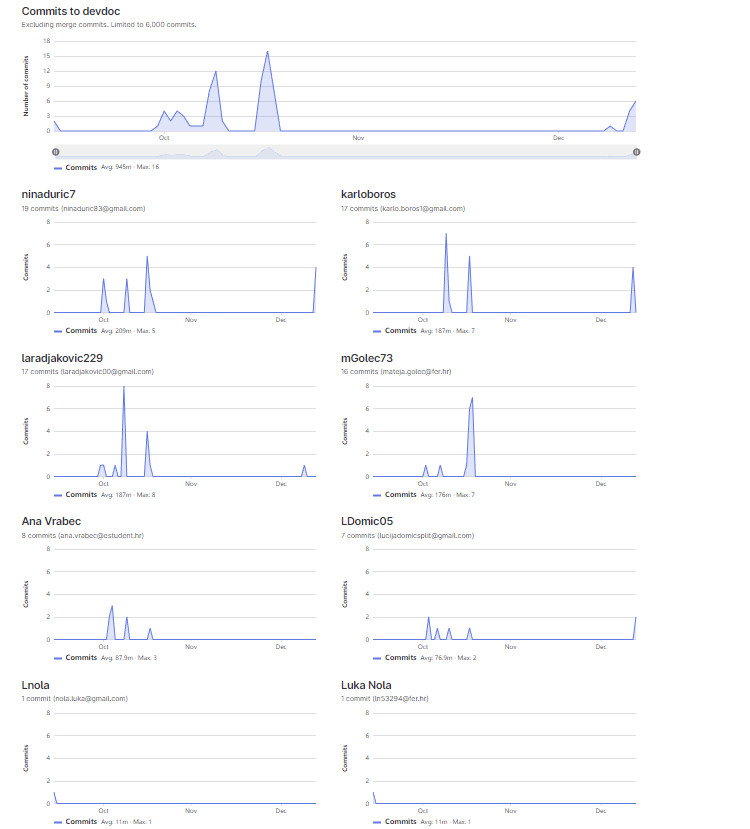
\includegraphics[scale=1.0]{slike/git6.png} %veličina slike u odnosu na originalnu datoteku i pozicija slike
			\centering
			\caption{Aktivnost devdoc grane}
			\label{fig:aktivnost6}
		\end{figure}
	